\errorcontextlines=5

%%%

\documentclass[
%handout,
]{beamer}

\usepackage{ifluatex}
\ifluatex\else\errmessage{This document requires LuaLaTeX}\fi

\usepackage{etex,etoolbox}
\usepackage{fontspec}
\usepackage[ngerman]{babel}
\usepackage{csquotes}
\usepackage{array}
\usepackage{wrapfig}
\usepackage{booktabs}
\usepackage{ccicons}
\usepackage{calc}

\usepackage{tikz}
\usetikzlibrary{arrows,intersections,calc,through,%
  external,positioning,automata,datavisualization,%
  datavisualization.formats.functions}

\usepackage{luacode}
\usepackage{pgfplots}
\usepackage{manfnt}

%%% title and such

\title{Wissenschaftliches Arbeiten mit \LaTeX}
\author{\texorpdfstring{Felix Hilsky\\basierend auf einem Kurs von\\Daniel Borchmann,\\Tom Hanika und \\Max Marx}{Felix Hilsky basierend auf einem Kurs von Daniel Borchmann, Tom Hanika und Max Marx}}
\titlegraphic{\ccLogo \ccAttribution \ccShareAlike}

%%% theme

\usepackage{tikz}
\usetikzlibrary{shapes.multipart}
\usetheme{CambridgeUS}
\setbeamertemplate{blocks}[rounded][shadow=false]
\setbeamertemplate{items}{\raisebox{0.3ex}{%
    \tikz[scale=0.13] \draw[fill] (0,0) -- (0,1) -- (0.9,0.5) -- cycle;}}
\usetikzlibrary{arrows}
\tikzset{>={stealth'[sep]}}
\setbeamertemplate{navigation symbols}{}
\setbeamertemplate{footline}{}
\setlength{\abovedisplayskip}{0pt}
\setbeamerfont{title}{series=\bfseries}
\defbeamertemplate{block alerted begin}{bends}{%
  \begin{columns}
    \begin{column}{0.05\linewidth}
      \dbend
    \end{column}
    \begin{column}{0.95\linewidth}
      \vskip.75ex\usebeamercolor[fg]{block title
        alerted}\insertblocktitle{}
      \vskip.1em
      \usebeamercolor[fg]{normal text}
}
\defbeamertemplate{block alerted end}{bends}{%
    \end{column}
  \end{columns}
}
%%%

\mode<handout>{
  \usepackage{pgfpages}
  \pgfpagesuselayout{2 on 1}[a4paper,border shrink=5mm]
}

%%% lecture organization

\usepackage{xparse}
\DeclareDocumentCommand \Lecture { m m }{%
  \lecture{#1}{#2}
  \part{#1}
  \include{#2}
}

\AtBeginSection{
  \setbeamertemplate{blocks}[rounded][shadow=true]
  \begin{frame}[plain]
    \begin{block}{}
      \begin{center}
        \textcolor{darkred}{\textbf{\Large \strut\smash{\insertpart}}}\\[1ex]
        \textcolor{blue!70!black}{\strut\smash{\insertsection}}
      \end{center}
    \end{block}
  \end{frame}
  \setbeamertemplate{blocks}[rounded][shadow=false]
  \setbeamertemplate{block alerted begin}[bends]
  \setbeamertemplate{block alerted end}[bends]
}

%%% misc

\newcommand{\GNULinux}{GNU\lower-0.25ex\hbox{/}Linux}
\newcommand{\TikZ}{Ti\emph{k}Z}

\usepackage{listings}

\lstset{language=[LaTeX]TeX, basicstyle=\ttfamily,
  keywordstyle={\color{blue}\bfseries}, frame=tb, extendedchars=true, literate=%
  {ä}{{\"a}}1 {ö}{{\"o}}1, escapeinside={(*@}{@*)}, mathescape=true,
  basewidth=0.5em, keywordstyle={\color{blue}},
  morekeywords={[0]includegraphics,rotatebox,scalebox,resizebox,providecommand,
    subsection,subsubsection,paragraph,subparagraph,part,chapter,tableofcontents,
    mathring,text,mathbb,printindex,addbibresource,printbibliography,subtitle,
    institute,titlegraphic,subject,keywords,draw,path,color,textcolor,toprule,
    midrule,bottomrule,maketitle,setlength,enquote,listoffigures,listoftables,
    theoremstyle,theoremheaderfont,theorembodyfont,newblock,parencite,footcite,
    autocite,bibitem,middle,tikzset,usetikzlibrary,coordinate,node,foreach,
    datavisualization,varepsilon,autocite,bibitem,DeclareRobustCommand,
    DeclareDocumentCommand,IfBooleanTF,bye,frametitle,setbeamertemplate,pause,
    onslide,uncover,visible,invisible,only,alt,temporal,alert,AtBeginSection,
    usetheme,setbeamerfont,tikz,includeonlyframes,mode,pgfpagesuselayout,RequirePackage,
  },
}

\AtBeginDocument{\frame[plain]{\maketitle}}

%%% end of preamble
\subtitle{Einführung}
\date{Sommersemester 2017}

\begin{document}

\section{Inhalt, Ablauf, Termine}
\begin{frame}[fragile]
  \frametitle{Inhalt}
  \setbeamertemplate{enumerate item}{\insertenumlabel.}
  \begin{enumerate}%[<+->]
  \item Grundidee und TeX-Editoren (und Installationshilfe)
  \item Dokumentenklassen, Pakete und Markup
  \item Mathematische Formeln
  \item Eigene Befehle
  \item Verweise, Tabellen, Bilder%Diagramme, 
  \item Literaturverzeichnisse% erstellen mit \LaTeX{}
  \item Formatierung
  \item Präsentationen erstellen mit \LaTeX{} (aka Beamer)
  \item Lua\LaTeX, Lua in \LaTeX
  \item Grafiken erstellen mit \LaTeX{} (aka tikz)
  \end{enumerate}
  \begin{itemize}
    \item permanent: Fehlersuche
  \end{itemize}
\end{frame}

\section{Fragen bis hierher?}

\section{Eine (sehr) kurze Geschichte von \LaTeX{}}
\begin{frame}\frametitle{Kurze Geschichte von \LaTeX{} I}

  \begin{columns}
    \begin{column}{0.7\linewidth}
      \begin{itemize}
      \item<1-> Von 1978 bis 1986 entwickelte \textsc{Donald E.\ Knuth} das
        Textsatzsystem \TeX{}.
      \item<2-> ΤΕΧΝΗ (technē) -- Kunst und Kunstfertigkeit
      \item<3-> keine Weiterentwicklung mehr
      \item<4-> der Quellcode ist \textit{frei}
      \item<5-> aktuelle Version ist 3.14159265
      \end{itemize}
    \end{column}
    \begin{column}{0.3\linewidth}
      \onslide<1->{%
        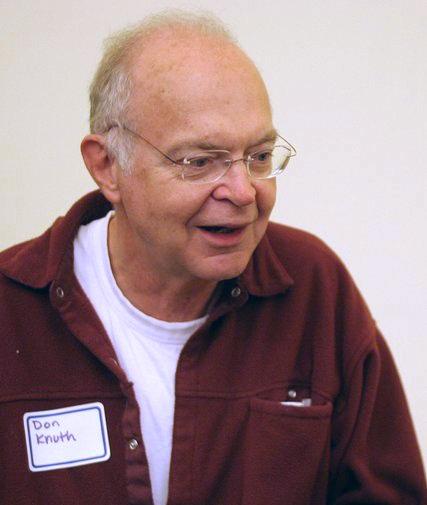
\includegraphics[width=3cm]{pics/KnuthAtOpenContentAlliance.jpg}
        \hspace*{0.05cm}%
        \rotatebox{90}{%
          \scalebox{0.25}{%
            \url{%
              http://commons.wikimedia.org/wiki/File:KnuthAtOpenContentAlliance.jpg}}}}
    \end{column}
  \end{columns}
\end{frame}

\begin{frame}\frametitle{Short history of \LaTeX{} II}

  \begin{columns}
    \begin{column}{0.7\linewidth}
      \begin{itemize}
      \item<1-> Beginn der 1980er Jahre entwickelte \textsc{Leslie
          Lamport} \LaTeX{} (also \textbf{La}+\TeX{}).
      \item<2-> 1990 endete seine Entwicklung an \LaTeX{} mit der Version 2.09.
      \item<3-> Seit 1990 wird an dem Nachfolger, \LaTeXe{} entwickelt.
      \item<4-> \LaTeX{} ist also \textbf{eine} Variante \TeX{} zu benutzen.
      \end{itemize}
    \end{column}
    \begin{column}{0.3\linewidth}
      \onslide<1->{%
        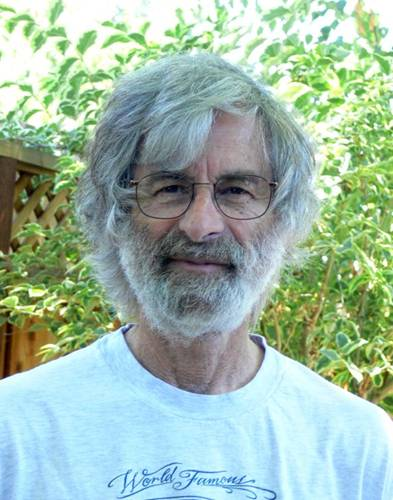
\includegraphics[width=3cm]{pics/Leslie_Lamport.jpg}
        \hspace*{0.05cm}%
        \rotatebox{90}{%
          \scalebox{0.25}{%
            \url{%
              http://upload.wikimedia.org/wikipedia/commons/5/50/Leslie_Lamport.jpg}}}}
    \end{column}
  \end{columns}
\end{frame}

\section{\TeX{} und \LaTeX{} verstehen}

\begin{frame}
  \frametitle{You see what you get?}
  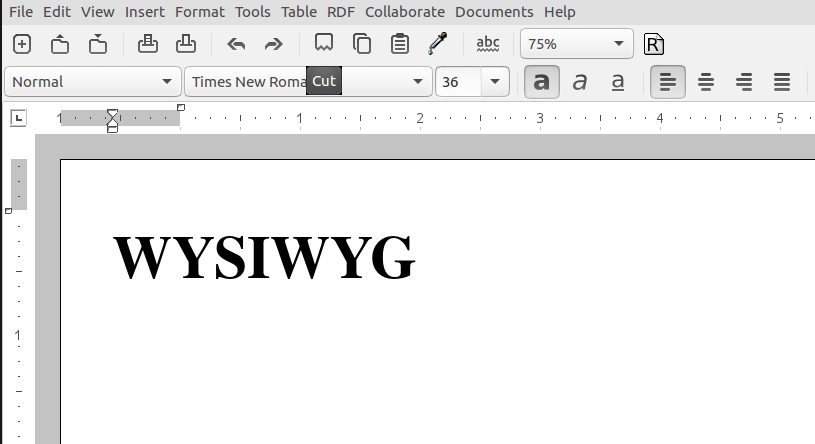
\includegraphics[width=\textwidth]{pics/wysiwyg.png}

  \textbf What \textbf you \textbf see \textbf is \textbf what \textbf you \textbf get.
\end{frame}

\begin{frame}
  \frametitle{You won't see what you get?}
  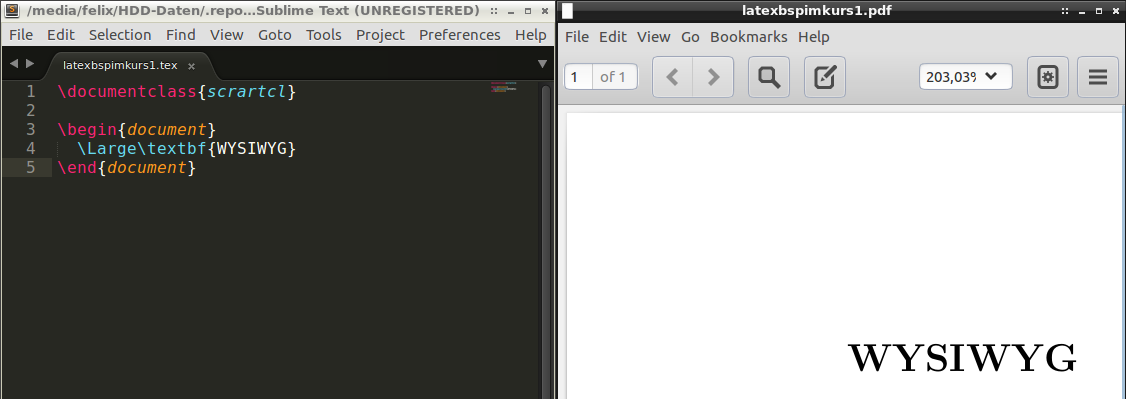
\includegraphics[width=\textwidth]{pics/wysiwyg2.png}
\end{frame}
\begin{frame}\frametitle{WYSIWYG}
  \begin{columns}
    \begin{column}{0.4\textwidth}
      \centering
      {\Large \enquote{verbreitete} Textverarbeitung}\\
      \ \\
      \onslide<1->{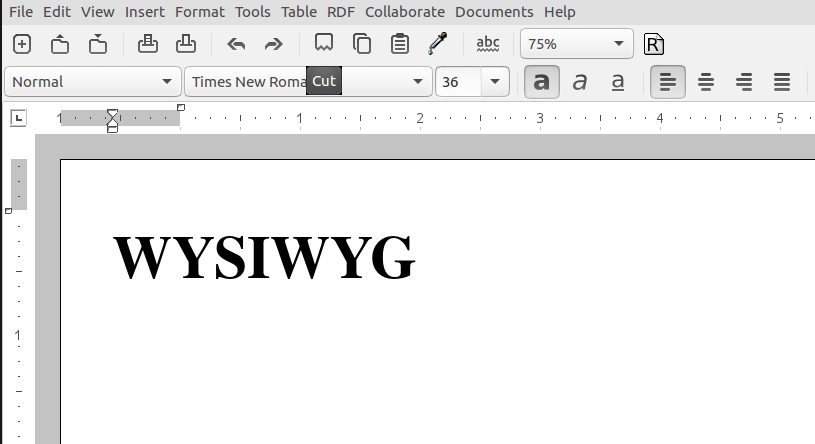
\includegraphics[width=\textwidth]{pics/wysiwyg.png}}
    \end{column}
    \begin{column}{0.6\textwidth}
      \centering
      {\Large\LaTeX{}}\\
      \ \\
      \onslide<1->{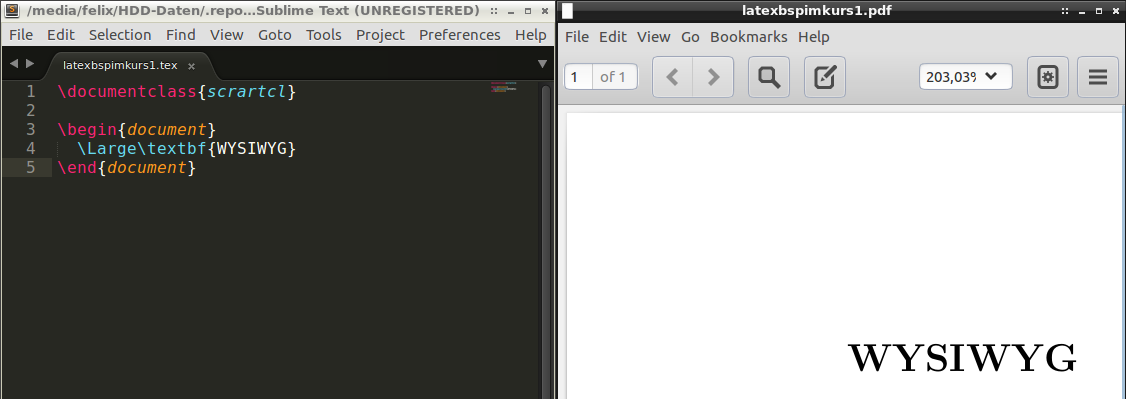
\includegraphics[width=\textwidth]{pics/wysiwyg2.png}}
    \end{column}
  \end{columns}

  \bigskip
  
  \onslide<2->

  \Large

  \LaTeX{} ist \textbf{WYSIWYM}.
  
\end{frame}

\begin{frame}
  \frametitle{Wir brauchen einen Text(datei)-Editor!}

  \onslide<+->

  \begin{block}{Merke!}
    \LaTeX-Dateien sind reine \emph{Textdateien}!
  \end{block}

  \onslide<+->
  
  Wir brauchen also einen Texteditor!

  \onslide<+->
  
  Es gibt eine riesige Menge von speziellen Text-Editoren für $*$\TeX{}\ldots. Bspw.\
  % 
  %  Die Wikipedia verzeichnet allein 44 Programme. Empfohlen seien die
  % folgenden:
  \begin{itemize}[<+->]
  \item TeXstudio (Free Software, Cross plattform)
  \item TeXmaker  (Free Software, Cross plattform)
  \item Kile      (Free Software, Unix-like only)
  \item vim mit LaTeX-suite
  \item TeXnicCenter (Free Software, Windows only)
  \item \textbf{Der GNU Emacs} mit der Erweiterung AUCTeX.
  % \item Bela nutzt: Sublime Text (leider nur gratis, nicht frei).
  \end{itemize}
\end{frame}

% \begin{frame}[fragile]
%   \frametitle{Was macht \LaTeX{}?}

%   \begin{tikzpicture}[node distance=0.5cm]
%     \only<2-3>{%
%       \node (c) [anchor=north west, rounded corners, fill=blue!20, draw] {%
%         \begin{tabular}{l}
%           \texttt{\textbackslash documentclass\{article\}}  \\
%           \texttt{\textbackslash begin\{document\}}\\
%           \texttt{Die Mathematik ist doch die angenehmste Wissenschaft.}\\
%           \texttt{\textbackslash end\{document\}}
%         \end{tabular}};
%     }
    % \only<beamer| beamer:3>{
    %   \node [below=of c, anchor=north, rounded corners, draw]{%
    %     \includegraphics[width=3cm]{pics/texex1.pdf}};
    % }
    % \only<beamer| beamer:4->{
    %   \node (x) [anchor=north, rounded corners, draw]{%
    %     \includegraphics[width=0.98\linewidth, clip, viewport=50 650 500 750]{%
    %       pics/texex1.pdf}};
    %   \node [anchor=north, rounded corners, draw, below=of x]{%
    %     \includegraphics[width=0.98\linewidth, clip, viewport=80 0 530 100]{%
    %       pics/texex1.pdf}};
    % }    
%     \only<handout>{pics
%       \node[below=of c, anchor=north] {%
%         \textrm{Die Mathematik ist doch die angenehmste Wissenschaft}};
%     }
%   \end{tikzpicture}
% \end{frame}

% \begin{frame}[fragile]
%   \frametitle{Was macht \LaTeX{}?}

%   \begin{tikzpicture}
%     \onslide<2-3>{%
%       \node (c) [anchor= north west, rounded corners, fill=blue!20, draw]{
%         \begin{tabular}{l}
%           \texttt{\textbackslash documentclass\{article\}}  \\
%           \texttt{\textbackslash usepackage\{amsmath\}}\\
%           \texttt{\textbackslash begin\{document\}}\\
%           \texttt{\ \ The formula is \$\textbackslash frac\{-b \textbackslash pm \textbackslash sqrt\{b\^{}2 - 4ac\}\}\{2a\}\$}\\
%           \texttt{\textbackslash end\{document\}}
%         \end{tabular}};}
%     \onslide<3-3>{\node [anchor=north west,below=of c,rounded corners, draw]{%
%         The formula is $\frac{-b \pm \sqrt{b^2 - 4ac}}{2a}$};}
%   \end{tikzpicture}
% \end{frame}

\begin{frame}[fragile]

  \onslide<+->

  \begin{block}{Wichtig!}
    \begin{center}
      \Large
      
      \textbf{Um \LaTeX{} nutzen zu können,\\ muss man nicht alles über \LaTeX{}
        wissen!}
    \end{center}

    Ein solides Grundwissen reicht für die meisten Anwendungen aus.
  \end{block}

  \onslide<+->

  \bigskip
  
  Weitere Hilfe:

  \begin{itemize}
  \item \verb|texdoc «Paket-oder-Klasse»|
  \item \href{http://ctan.org}{CTAN} (Comprehensive \TeX{} Archive Network)
  \item DAS INTERNET
  \item Lokale \TeX\ User-Group (\url{http://tug-dd.kxpq.de})
  \end{itemize}
  
\end{frame}

% \begin{frame}[fragile]
%   \frametitle{Jetzt geht es los!}
% \begin{lstlisting}
% \documentclass[ngerman]{scrartcl}   % Dokumententyp

% \usepackage[T1]{fontenc}            % Schriftkodierung
% \usepackage[utf8]{inputenc}         % Eingabekodierung
% \usepackage{babel}                  % Sprachunterstützung

% \title{Mein erstes \LaTeX-Dokument} % Titel
% \author{Das ist von mir!}           % Autor
% \date{Stardate 47943.2}             % Datum

% \begin{document}                    % Ab hier kommt Inhalt

% \maketitle                          % Autom. Titel

% Das ist ja einfach!                 % Inhalt
% \end{document}                      % Ende
% \end{lstlisting}

% \end{frame}

\end{document}

%%% Local Variables:
%%% mode: latex
%%% TeX-engine: luatex
%%% TeX-master: t
%%% End:
